% LaTeX Template for Project Report, Version 2.0
% (Abstracted from a Major Project Report at CSED, NIT Calicut but can be
% modified easily to use for other reports also.)
%
% Released under Creative Commons Attribution license (CC-BY)
% Info: http://creativecommons.org/licenses/by/3.0/
%
% Created by: Kartik Singhal
% BTech CSE Batch of 2009-13
% NIT Calicut
% Contact Info: kartiksinghal@gmail.com
%
% It is advisable to learn the basics of LaTeX before using this template.
% A good resource to start with is http://en.wikibooks.org/wiki/LaTeX/
%
% All template fields are marked with a pair of angular brackets e.g. <title here>
% except for the ones defining citation names in ref.tex.
%
% Empty space after chapter/section/subsection titles can be used to insert text.
%
% Just compile this file using pdflatex after making all required changes.

\documentclass[12pt,a4paper]{report}
\usepackage[pdftex]{graphicx} %for embedding images
\usepackage{url} %for proper url entries
\usepackage{booktabs}
\usepackage[acronym, toc]{glossaries}
\usepackage[colorinlistoftodos]{todonotes}
\usepackage[bookmarks, colorlinks=false, pdfborder={0 0 0}, pdftitle={<MEng Individual Project Interim Report>}, pdfauthor={<Yangfan Zhang>}, pdfsubject={<Computing>}, pdfkeywords={<TFL, Bus Arrival Times, Delay>}]{hyperref} %for creating links in the pdf version and other additional pdf attributes, no effect on the printed document
%\usepackage[final]{pdfpages} %for embedding another pdf, remove if not required

\makeglossaries
%!TEX root = report.tex


\begin{document}
\renewcommand\bibname{References} %Renames "Bibliography" to "References" on ref page

%include other pages
\begin{titlepage}

\newcommand{\HRule}{\rule{\linewidth}{0.5mm}} % Defines a new command for the horizontal lines, change thickness here

\center % Center everything on the page
 
%----------------------------------------------------------------------------------------
%	HEADING SECTIONS
%----------------------------------------------------------------------------------------

\textsc{\LARGE Imperial College London}\\[1.5cm] % Name of your university/college
\textsc{\Large Department of Computing}\\[0.5cm] % Major heading such as course name
\textsc{\large MEng Individual Project Interim Report}\\[0.5cm] % Minor heading such as course title

%----------------------------------------------------------------------------------------
%	TITLE SECTION
%----------------------------------------------------------------------------------------

\HRule \\[0.4cm]
{ \huge \bfseries Active Delay Warning Transport App}\\[0.4cm] % Title of your document
\HRule \\[1.5cm]
 
%----------------------------------------------------------------------------------------
%	AUTHOR SECTION
%----------------------------------------------------------------------------------------

\begin{minipage}{0.4\textwidth}
\begin{flushleft} \large
\emph{Author:}\\
Yangfan \textsc{Zhang} % Your name
\end{flushleft}
\end{minipage}
~
\begin{minipage}{0.4\textwidth}
\begin{flushright} \large
\emph{Supervisor:} \\
Dr. Peter \textsc{McBrien} % Supervisor's Name
\end{flushright}
\end{minipage}\\[4cm]
% If you don't want a supervisor, uncomment the two lines below and remove the section above
%\Large \emph{Author:}\\
%John \textsc{Smith}\\[3cm] % Your name

%----------------------------------------------------------------------------------------
%	DATE SECTION
%----------------------------------------------------------------------------------------

{\large \today}\\[3cm] % Date, change the \today to a set date if you want to be precise

%----------------------------------------------------------------------------------------
%	LOGO SECTION
%----------------------------------------------------------------------------------------

%\includegraphics{Logo}\\[1cm] % Include a department/university logo - this will require the graphicx package
 
%----------------------------------------------------------------------------------------

\vfill % Fill the rest of the page with whitespace

\end{titlepage}
%!TEX root = report.tex
\vspace{2in}
\begin{abstract}
\todo[inline]{abstract}
<Abstract here>
The abstract is a very brief summary of the report's contents. It should be about half a page long. Somebody unfamiliar with your project should have a good idea of what it's about having read the abstract alone and will know whether it will be of interest to them. Note that the abstract is a summary of the entire project including its conclusions. A common mistake is to provide only introductory elements in the abstract without saying what has been achieved.

\end{abstract}
%!TEX root = report.tex
\cleardoublepage
%\pagebreak
\phantomsection
\addcontentsline{toc}{chapter}{Acknowledgements}
\chapter*{Acknowledgments}
\vspace{1.0in}
<Acknowledgements here>
Peter McBrien, Susan
\\
\\
\\
\\
<Name here> \\
\\
\\
<Month and Year here>\\
{National Institute of Technology Calicut}\\
\newpage

\pagenumbering{roman} %numbering before main content starts
\tableofcontents
\listoffigures

\newpage
\pagenumbering{arabic} %reset numbering to normal for the main content

%\input{./prob-definition.tex} %objective changed to problem definition
%!TEX root = report.tex
\chapter{Introduction}

The London bus network carries 2.4 billion passengers a year, more than the rest of England combined \cite{tfl_annual_report_13/14}.

\par The bus arrival times published by Transport for London (TfL) are currently widely available on digital live bus arrivals signs at more than 2,500 bus stops \cite{live_bus_arrivals}. Passengers can also check this information by sending a text message with the bus stop code, as well as doing a quick search online or on mobile applications.

\todo[inline]{Passengers chose travel mode based on travel time and convenience. Find evidence for this assumption. How do people choose travel mode / whether to take bus? }

\todo[inline]{Scenario, a passenger chose to take a bus, then only realises delay at the end of the journey. Would have chosen another mode of travel should he know of the delay earlier.}

\par Passengers rely on the bus arrival times to plan their journey, by factoring in the waiting time when choosing the buses to take. Current London journey planning software takes the journey start time, start location, and destination as input, and recommends routes consisting of a variety of travel mode, with an estimate travel time for each suggested journey. Such popular planners include Google maps \cite{google_maps}, Citymapper \cite{citymapper} and Transport for London Journey Planner \cite{tfl_journey_planner}.

\par However, the accuracy of the bus arrival times published is affected by many external factors. For example, when there is heavy traffic, the buses are likely to be delayed by a difference significant enough for a change in passengers' route picking. Yet, this delay information is not reflected in the arrival time data or the estimated journey time early enough for the passengers to make a decision to choose an alternate route. As a result, passengers waste time waiting for buses that come much later than expected, or chosing to board a bus that takes far longer than the estimated journey time. Although the average bus delay is 1 minute, there was a 16.6 chance of waiting for more than 10 minutes \cite{buses_performance_data}.

\par This can be avoided if passengers are informed of the delays in bus arrival times in advance. Such delays can predicted by analysing the historical delays. This is achieved by collecting data from the Transport for London live bus arrivals API stream feed\cite{live_bus_arrivals}, and estimate the average journey time required between two locations on a given time of the day. Next, a bus arrival time table with delays during various time windows over a week can be crafted and fine tuned incrementally. We compared the travel times in this timetable with the official travel times published by the Transport of London Open Data to find out the delays in bus arrival times.
%!TEX root = report.tex
\chapter{Background}

\section{London Bus Network}

\par The bus network in London is one of the largest and most accessible in the world. It is carrying a staggering number of passengers, with more than 2.4 billion journeys in 2013/14, which was more than any year since 1959 \cite{tfl_annual_report_13/14}.

\par On an average day between 2005 and 2010, about 14\% of the trips made by London residents were by bus \cite{tfl_ltds}. They spent on average 14 minutes per day on these bus trips.

\par There are currently 19,345 bus stops, and 680 routes served by 8,765 buses daily in London\cite{bus_stop_locations_routes}.

\todo[inline, color=purple]{produce graph for this, number of stops, routes and buses}
% number of people that use apps to plan journey or pick the bus to take

\subsection{Bus Network Performance}

\par TfL published the following figures in the second quarter 2014/2015 buses performance data \cite{buses_performance_report}.

\par For the high frequency services, the average scheduled wait was 4.86 minutes, the average excess wait was 0.94 minutes, and the average actual wait was 5.80 minutes. While passengers could expect the buses to come within 10 minutes 83.4\% of the time, there was 15.1\% chance of waiting for 10-20 minutes, 1.3\% chance of waiting for 20-30 minutes, and 0.2\% chance of waiting for more than 30 minutes.

\par For the low frequency services, 87\% of the buses services were on time, and 11.4\% were 5-15 minutes late.

\par For the night buses, 84.5\% of the services were on time. The average excess wait was 0.68 minutes.

\todo[inline, color=purple]{produce graph here}

\par The bus arrivals might be affected by traffic congestion, staff availability, engineering problems, or mechanical breakdown \cite{buses_performance_data}.

\section{Buses Status Updates}
\par To inform passengers of the bus service disruptions or diversions, \acrshort{tfl} provides a bus status updates service online \cite{tfl_buses_status_updates}. Passengers can retrieve relevant bus service status for a given bus stop or route (Figure \ref{fig:tfl_status_update}).

\begin{figure}
\centering
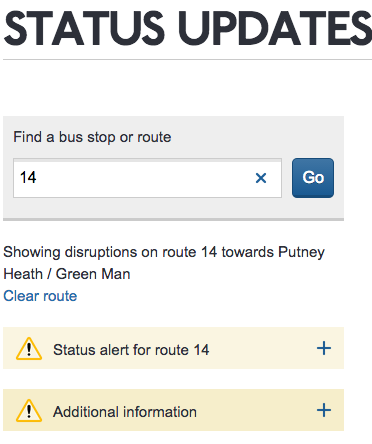
\includegraphics[width=0.5\textwidth]{figures/tfl_status_update.png}
\caption{\label{fig:tfl_status_update} Tfl Buses Status Update Service}
\end{figure}

\par The textual information include service disruptions, diversion, suspensions, and delays due to heavy traffic.

\par While this service informs passengers of current abnormal bus schedules, it requires passengers to visit the site to check for specific information, and does not provide an estimation on the travel time under the special conditions.

\par \acrshort{tfl} also publishes live status news and updates on Twitter \cite{tfl_bus_alerts_twitter}, but it is not easily searchable by passengers to check specific information relevant to their journeys.

\par Additionally, many current popular journey planners such as Google Maps\cite{google_maps}, Citymapper London\cite{citymapper}, and \acrshort{tfl} Journey Planner incorporate the bus delay information in the suggested journeys as a textual alert. These apps do not recompute the estimated journey time for passengers to make an informed decision.

\par As a result, the lack of data service on bus delay predictions and travel times



. This presents a significant barrier to bus passengers who wish to plan their bus journeys for specific appointments.

\section{Choice of Travel Mode}
\todo[inline]{Does the arrival time / delay affect people's choice of travel mode? What are the purposes of commute? Work, travel, leisure, appointments?}

%!TEX root = report.tex
\section{Transport for London Open Data}
\acrshort{tfl} provides data to quantify the delays in bus journey time. We collected the necessary data from the Live Bus Arrivals \acrshort{api}, Bus Stop Locations and Routes, and Journey Planner Bus Timetables. The Live Bus Arrivals \acrshort{api} enables a query to receive a bespoke response, depending on the parameters supplied. Bus Stop Locations and Routes come as static data files which rarely change. Journey Planner Bus Timetables are feeds that refresh at regular intervals.

%!TEX root = report.tex
\subsection{Live Bus Arrivals API Stream}
\par The Live Bus Arrivals API Stream provides the predicted time until a bus is expected to arrive at a stop. These predictions are available for the next 30 minutes at any point in time. For example, at 9am, the stream will provide predicted bus arrivals up to 9.30am on the same day. This data is refreshed every 30 seconds \cite{live_bus_api_documentation}.

\par The base URL is \url{http://countdown.api.tfl.gov.uk/interfaces/ura/stream_V1}. In order to collect bus arrival data for analysis, we supplied the following parameters which specify the fields returned by the \acrshort{api}.



%!TEX root = report.tex
\subsection{Bus Stop Locations and Routes}
\par The TFL Open Data provides network information on the location of all bus stops in London, and the sequence of bus stops in every bus route.

\par This data is in the comma-separated values (CSV) format. We imported the bus sequences into the delay\_bus\_sequences table (Table \ref{table:delay_bus_sequences})

\begin{table}
\centering
\begin{tabular}{@{}llr@{}} \toprule
Column Name & Type & Comments\\ \midrule
id(Primary Key) & int(11)  & Auto Increment\\
route & varchar(64) &  The route name\\
run & int(11) & The route direction\\
sequence & int(11) & The sequence of the bus stop in the route\\
stop\_code\_lbsl & varchar(64) & The internal bus stop identifier\\
bus\_stop\_code & varcher(64) & The public code for the bus stop\\
naptan\_atco & varchar(64) & The national identifier of the bus stop\\
stop\_name & varchar(64) & The name of the bus stop\\ \bottomrule
\end{tabular}
\caption{delay\_bus\_sequences Table Schema}
\label{table:delay_bus_sequences}
\end{table}
 \todo[inline, color=cyan]{Question: Can I skip some columns of the table schema, as those columns have not been used in the project, but just storing as reference for now?}
\par Additionally, we extracted information on all pairs of neighbouring bus stops and the routes that serve between them. We save this information in the delay\_neighbours table (Table \ref{table:delay_neighbours}). See sample data in Table \ref{table:sample_neighbours_view}.

\begin{table}
\centering
\begin{tabular}{@{}llr@{}} \toprule
Column Name & Type & Comments\\ \midrule
id(Primary Key) & int(11)  & Auto Increment\\
route & varchar(64) & The bus route \\
start\_stop & varchar(64) & The stop\_code\_lbsl for the start stop\\
end\_stop & varcher(64) & The stop\_code\_lbsl for the end stop\\ \bottomrule
\end{tabular}
\caption{delay\_neighbours Table Schema}
\label{table:delay_neighbours}
\end{table}

\begin{table}
\centering
\begin{tabular}{@{}llrr@{}} \toprule
id & route & start\_stop & end\_stop \\ \midrule
18433 & 30 & 10002 & 11469 \\
44878 & N19 & 10002 & 11469 \\
47128 & N41 & 10002 & 29772 \\
8653 & 19 & 10002 & 11469 \\ \bottomrule
\end{tabular}
\caption{Sample data in delay\_neighbours Table}
\label{table:sample_neighbours_view}
\end{table}

\subsubsection{Finding the average travel time between neighbouring stops}
\todo[inline] {update this part}
\par To experiment with the queries, we selected one pair of the neighbouring stops (10002, 11469), and listed the time required to travel from stop 10002 to stop 11469 by finding the difference in arrival times for each journey. Sample entries of this list is shown in Figure \ref{fig:journey_time_10002}.

\begin{figure}
\centering
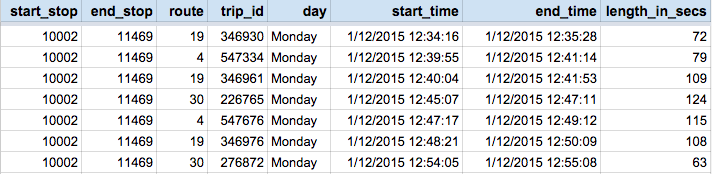
\includegraphics[width=0.7\textwidth]{figures/journey_time_10002.png}
\caption{\label{fig:journey_time_10002} List of journey time from stop 10002 to stop 11469}
\end{figure}


\par We then calculated the average journey time required to travel from 10002 to 11469 for each hour in each week of the day. This information is stored as a timetable, which would be used for further analysis.

Figure\ref{fig:timetable_10002} shows the timetable generated. Each cell indicates the average journey time required to travel from stop 10002 to stop 11469 at a give hour of a give week of day. The \textbf{NULL} values are due to a current databases performance issue. This will be resolved later.

\begin{figure}
\centering
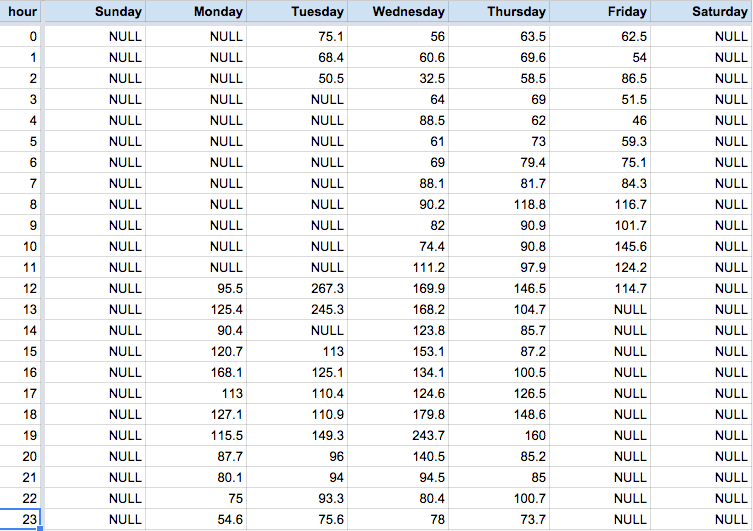
\includegraphics[width=0.9\textwidth]{figures/timetable_10002.png}
\caption{\label{fig:timetable_10002} Average journey time in seconds from stop 10002 to stop 11469 for each hour of each day of week}
\end{figure}

\par We plan to construct a timetable this way for each pair of the neighbouring bus stop.
%!TEX root = report.tex
\subsection{Journey Planner Bus Timetables}
The Journey Planner Bus Timetables \cite{open_data_feeds_description} contains information on official bus schedules including stops, routes, departures times, departure frequencies, operational notes, as well as the days on which the services run.

The timetables uses the \acrfull{xml} \cite{xml} format, with the schema defined in \gls{transxchange} \cite{transxchange}, the UK nationwide standard for exchanging bus schedules and related data. For this project, we used the General schema version 2.1\cite{transxchange_downloads_and_schema}\cite{transxchange_schema_2.1_xsd}, the latest available version for download. Each \acrshort{xml} file contains the bus timetables for one route. Figure \ref{fig:xml_components} shows the overview of a timetable \acrshort{xml} file.

\begin{figure}
\centering
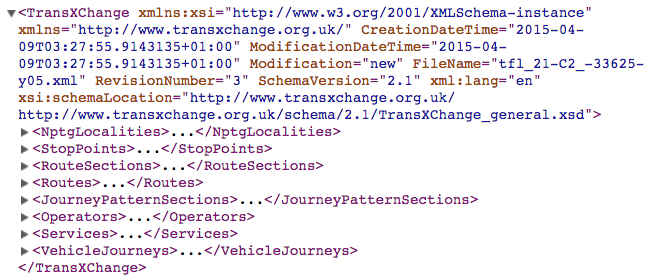
\includegraphics[width=1\textwidth]{figures/xml_components.png}
\caption{\label{fig:xml_components} TfL Journey Planner Timetables Sample XML Overview}
\end{figure}

\subsubsection{Data Structure}
The \gls{transxchange} timetable model has the following seven basic concepts\cite{transxchange_schema_guide}:

\begin{enumerate}
  \item \texttt{Service} contains one or more \texttt{JourneyPattern} elements and one or more \texttt{VehicleJourney} elements. This is the basic concept that brings together the information about a registered bus service.
  \item \texttt{Registration} specifies the registration details for a service.
  \item \texttt{Operator} indicates the entity who runs the service.
  \item \texttt{Route} describes the physical path taken by buses on the service as an ordered list of \texttt{StopPoints}.
  \item \texttt{StopPoint} contains reusable declarations of the stops used by the routes and journey patterns of the schedule. All StopPointRef instances elsewhere in a document are resolved against the contents of the StopPoints element. All stops are defined as being \gls{naptan} points.
  \item \texttt{JourneyPattern} specifies an ordered list of links between the \texttt{StopPoints}, giving the \emph{relative travel times} between each pair of neighbouring stops.
  \item \texttt{VehicleJourney} specifies the individual scheduled journey \emph{at a specific absolute time}.
\end{enumerate}

These elements give a complete official bus schedule for each route with the departure time for each bus journey, the relative bus travel time between stops, and the days on which the service operates on. We extracted the official bus timetables from these \acrshort{xml} files, as discussed in Section \ref{sec: official_tfl_timetable}.

% %!TEX root = report.tex
\subsection{iBus System}
The actual arrival time of buses on a route at any given bus stop for the selected day are made available by the London Buses iBus system.

Currently, the routes were selected as the first of the New Routemaster (New Bus for London). Data will be published once a week \cite{buses_performance_data}.

This data is stored in comma-separated values (CSV) format. There are two potential uses for this data.
\begin{itemize}
	\item We can integrate it into the arrivals table to improve the precision of the arrivals data. Since the current entries in the arrivals table contain estimated bus arrival times, the integrated of the iBus data which contains real bus arrival times will likely boost the precision of the data in arrival table.
	\item We can compare the predicted delays with the iBus data for performance evaluation.
\end{itemize}

\section{Additional Background Materials}
Here's a list of the potential points to be covered in the final report.

\begin{itemize}
	\item Geocoding data
    \item Possible analysis methodologies such as regression
    \item Literature review on similar research done in other areas of the world
\end{itemize}

\todo[inline]{document a service that other developers can use, with demo app to show the features}
\todo[inline]{background on other apps}
\todo[inline]{document the DB}


% \section{Other Available Data}
% \subsection{Greater London Data}
% \subsection{Geocoding}

% \section{Analysis Methodologies}
% % \todo[inline]{I am not really sure what methods to use for analysis}
% \subsection{Regression}
% \subsection{Statistical Analysis}

% \section{Literature}
% \subsection{TFL Journey Planner}
% The website’s Journey Planner and homepage
% status board have also been redesigned and
% integrated so customers planning their trip can
% see immediately if their route is likely to be
% affected by upgrade work or other disruptions.
% The Journey Planner will now automatically
% generate cycling and walking routes, giving
% people a wider range of options for their journey \cite{tfl_annual_report_13/14}

% \subsection{Google Maps}
% \subsection{City Mapper London}


%!TEX root = report.tex
\subsection{Summary on Available Data}
\par While there is sufficient data on London bus network, official bus timetables, and live arrival times, there is no data service offering real-time predictions on bus delays.

\par \acrshort{tfl} releases information on service disruption, yet this is not incorporated


There is also a status updates service for passengers to check disruptions on the given bus stop or route.


%!TEX root = report.tex
\section{Current Travel Applications}

\begin{figure}
\centering
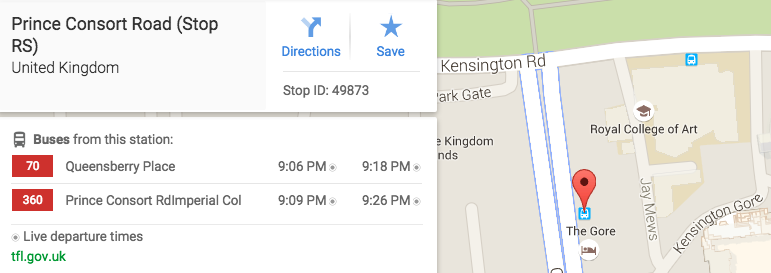
\includegraphics[width=1\textwidth]{figures/google_maps_tfl_data.png}
\caption{\label{fig:google_maps_tfl_data} Google Maps Using TfL Bus Arrival Data}
\end{figure}

Over 5,000 developers have registered for the open data\cite{open_data}, and around 200 travel apps are powered by it \cite{tfl_annual_report_13/14}. The most popular travel applications include \acrshort{tfl} Journey Planner, Google Maps (Figure \ref{fig:google_maps_tfl_data}), and Citymapper London. Given the departing location, destination, as well as departure time, these applications can provide suggested routes and travel times. Users can further customise their desired journey by specifying the desired walking distance, and accessibility requirements. Moreover, the \acrshort{tfl} Journey Planner and homepage
status board were redesigned and integrated so customers planning their trip can see immediately if their route is likely to be affected by upgrade work or other disruptions \cite{tfl_annual_report_13/14}, with a textual warning message shown.

\par However, currently, there are no applications that give predictions on travel times and warnings on potential delays. The estimated travel time shown in apps is extracted from the \acrshort{tfl} Journey Planner Bus Timetables. This information does not capture the real time delays according to instant traffic conditions.

%!TEX root = report.tex
\section{Literature}
\label{sec:literature}
\subsection{Overview}
\par We did some literature review on the conventional methods used to predict bus arrival times. They include regression models, Kalman filters models, \acrfull{ann} models, K-nearest neighbours models, and analytical approaches.

\subsection{Regression}
\par Regression estimates the relationship between a dependent variable and one or more independent variables. It was used by Patnaik et al. (2004) to predict bus arrival times to downstream stops with data collected by the \acrfull{apc} \cite{regression_models}.

\par The regression models require the independent variables to be uncorrelated to each other. It is difficult to provide such a set of variables in the context of bus arrivals predictions. This is because most of the independent variables are correlated (e.g. the number of intermediate bus stops and the number of signalised inter-subsections). Therefore, defining a set of uncorrelated independent variables is the main challenge of building regression models.

\subsection{Artificial Neural Network (ANN)}
\par \acrshort{ann} models are used to estimate functions that can depend on a large number of inputs by adjusting their parameters through message passing between neuron layers. An \acrshort{ann} model is trained with training examples including dependent variables and prediction results. The advantage of ANN is that the variables can be correlated, whereas the main disadvantage is that the model training process can take very long (more than 10 hours). Mazloumi (2009) built an artificial neural network with data collected by the Sydney Coordinated Adaptive Traffic System at intermediate signalised inter-subsections and schedule adherence to predict bus travel time \cite{ann}.

\subsection{Kalman Filters}
\par The Kalman filter, also known as linear quadratic estimation (LQE), is a linear recursive predictive algorithm. It starts with a primary estimate and allows parameters to be tuned with each new measurement, in order to find the optimal estimates of unknown variables \cite{kalman_filters}. It can respond to dynamic conditions of a modelled process, and has been used for dynamic travel time prediction models. Chen \textit{et al.} (2005) used Kalman filters to predict arrival time with taking into account the effect of schedule recovery impact \cite{kalman_dynamic_schedule}.

\subsection{K-Nearest Neighbours Regression (KNN)}
\par \acrfull{knn} regression algorithm takes in the \textit{k} closest training examples and produces an output of the property value based of the average of the values of its neighbours. Baker C. M. and Nied A. C. (2013) created models to predict arrival times using \acrshort{knn}, Kernel Regression and seven sets of features~\cite{knn_one_bus_away}.

\subsection{Analytical Approaches}
\par Analytical approaches are usually developed based on specific available data sets or special conditions. For example, Sun et al.(2007) proposed an algorithm that first tracks the bus to obtain the distance to each bus stop, and then predicts bus arrival time using the average speed in various temporal and spatial segmentation \cite{analytical_approach}.

\subsection{Summary on Literature Review}
\par Methods such as Regression, ANN, KNN and Kalman Filters mainly focus on defining and collecting information on factors that will cause a change in the bus journey time. The information is then processed to produce a prediction. Such factors include weather conditions, passenger flow, distance between bus stops, and the speed of the bus vehicle, etc.

Given the large size of London bus network, predicting bus journey times by discovering and analysing these factors is complicated as there are a lot of uncertainties on the road, and there is measuring error for each data point for each factor in consideration.

Since we needed to collect data for analysis and build the prediction model from scratch, we decided to use an analytical approach which is developed based on specific available data sets (\acrshort{tfl} Live Bus Arrivals), and is relatively simpler to implement at this stage. The other methods can be used to fine-tuned the prediction accuracy as future work.





%!TEX root = report.tex
\chapter{Concept Design}
\section{Objectives}
\par We aim to improve the prediction of bus travel time downstream from location of last observation in mixed traffic operations. We achieve this by providing an API data service of bus travel time predictions, and a demonstrative web application to show case the use of such a data service.

\section{Bus Travel Times}
\par The bus travel time between 2 neighbouring stops depends on many unpredictable external factors. These include weather conditions, passenger flow, temporary lane closures, as well as the time of the bus trip. Predicting bus travel times by discovering and analysing these contributing factors is complicated.

\par We decided to bypass looking at these factors, and examine the historical and current bus travel times instead. We assumed that for a specific short time frame, the external factors remain largely unchanged. In this case, the bus travel time between the given 2 neighbouring stops is similar to the previous trips performed in the same time frame.

\par For bus travel time between every pair of neighbouring stop at each hour of the day, we provide estimations for the following:
\begin{itemize}
  \item \textbf{Reference Timtable} How long does TfL says it take?
  \item \textbf{Current Timetable} How long does it currently take?
  \item \textbf{Historical Timetable} How long does it usually take?
\end{itemize}

\par Since the reference timetable shows the typical bus travel time, the historical timetable should converge to the reference timetable over time.

\par The current timetable shows the most relevant bus travel time at the observation point, a significant increase in travel time compared to the historical or refernece timetables would indicate a bus delay.

\subsection{Reference Timetable}
\par We extracted the average bus travel time between every pair of neighbouring stops for every route during every hour of the day for every day of the week from the \acrshort{tfl} Journey Planner Bus Timetables. This is discussed in Section \ref{sec: official_tfl_timetable}.

\subsection{Current Timetable}
\par We collect the live bus arrival times for the past 1 hour, and store the final bus arrival times for each bus at each stop. We then find out the travel time of each bus between every pair of neighbouring stops for the given hour. Next, we calculate the average travel time between each pair of neighbouring bus stops. This serves as a prediction for how long the bus currently takes to travel between two neighbouring stops. See implementation details in Section \ref{sec:current_timetable_generation}.

\subsection{Historical Timetable}
\par We store the current timetable generated at each hour, and group them by the hour of the day for the same day of the week. We then calculate the average bus travel time between each pair of neighbouring stops for each hour of the day in each day of the week. For example, the average bus travel time between stop A and stop B for 3pm on Wednesday is the average travel time for all the bus trips between these two stops between 2pm to 3pm in the past Wednesdays. More details cound be found in Section \ref{sec:historical_timetable}.

\section{Contributions}
\par We provided the above mentioned three timetables as an API data service (Chapter \ref{ch:data_service}) and designed a demostrative mbile application that warns users of current bus delays from a given bus stop (Chapter \ref{ch:mobile_app}).


\section{Architecture Design}
\begin{itemize}
\item Used Django Framework to build the backend that retrieves data from a MySQL database.

\item Used AngularJS with Twitter Bootstrap for frontend development
\end{itemize}
\missingfigure{graph to show the overall structure}






%!TEX root = report.tex
\chapter{Data Collection and Generation}
\label{ch:data_generation}
\section{Overview}
\begin{figure}
\centering
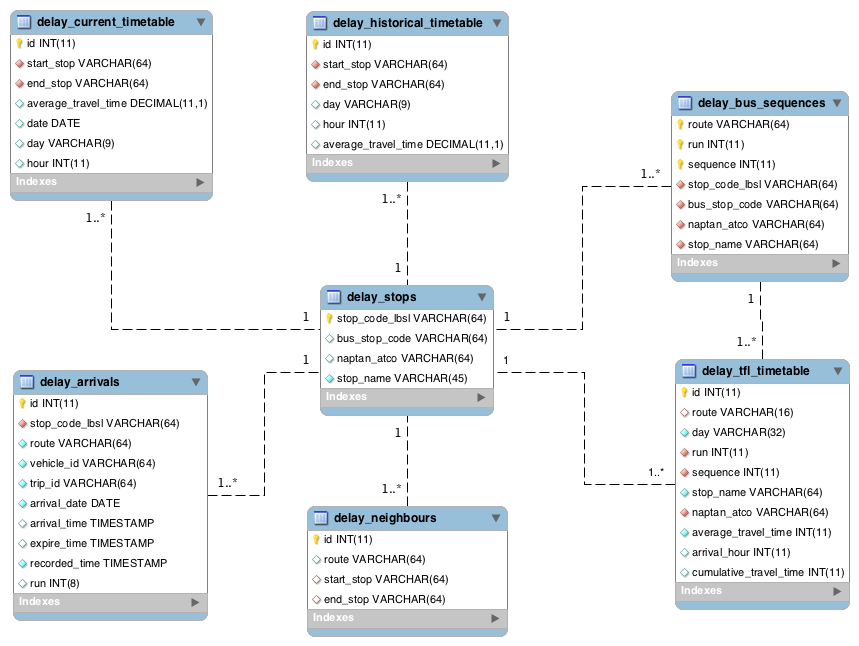
\includegraphics[width=\textwidth]{figures/uml.png}
\caption{\label{fig:uml} Databases Overview}
\end{figure}

\par This chapter discusses the backend development environment, and the detailed data collection and processing steps to generate the reference, current, and historical timetables. Figure \ref{fig:uml} shows the main tables in the Databases. We discussed the generation of these tables in the following sections.

\section{Development Environment}
\subsection{Virtual Machine}
\par We set up a Virtual Machine in the Doc's Private Cloud\cite{private_cloud} with the specifications shown in Table \ref{table:virtual_machine}. We allocated a large memory for memory intensive Databases operations.

\begin{table}
\centering
\begin{tabular}{@{}lr@{}} \toprule
Spec & Value \\ \midrule
Number of CPU Cores & 8 \\
CPU (in MHz) & 1000 \\
Memory (in GB) & 30 \\
 \bottomrule
\end{tabular}
\caption{Virtual Machine Specifications}
\label{table:virtual_machine}
\end{table}

\subsection{MySQL Databases}
\par We chose MySQL for backend data storage for the following reasons:

\begin{itemize}
  \item \textbf{User Interface} MySQL has convenient database management tools that enable easy data browsing, such as phpMyAdmin\cite{phpmyadmin} and Sequel Pro \cite{sequel_pro}.
  \item \textbf{Scalability} MySQL can handle memory-intensive computations efficiently once configured correctly.
\end{itemize}

\subsubsection{Databases Optimisation}
\par As some database operations involved joining large tables, we optimised the databases with the following settings in file \textit{/etc/mysql/my.cnf} to allow MySQL to access more memory in the Virtual Machine \cite{setting_innodb_buffer_pool_size,innodb_buffer}.

\begin{verbatim}
[mysqld]
innodb_io_capacity = 2000
innodb_read_io_threads = 64
innodb_thread_concurrency = 0
innodb_write_io_threads = 64
innodb_buffer_pool_size=20G
join_buffer_size=2G
sort_buffer_size=1G
read_buffer_size=1G
read_rnd_buffer_size=1G
max_connection=200
\end{verbatim}



%!TEX root = report.tex
\section{Generating Reference Timetable}
\label{sec: official_tfl_timetable}
For each day of the week, there are a predefined number of running the give route. We used the \texttt{VehicleJourneys} as a starting point to retrieve the departure time of the actual vehicle from the terminal. We then retrieved the corresponding \texttt{JourneyPattern}, and obtained the travel time between each neighbouring stops on the route for the given vehicle journey, to compute the cumulative travel times throughout the route.

The above computation was performed on each XML file to generate the actual arrival time and travel time for each vehicle trip at each stop in the route throughout the day. We grouped the bus travel time by the hour that the arrival time falls in, and find the average bus travel time between every pair of the neighbouring stops for the given hour of the given day of the week. The results of this computation was stored in the \texttt{delay\_tfl\_timetable} table (Table \ref{table:delay_tfl_timetable}).

\subsection{Detailed Steps}

\par We used the \texttt{ElementTree} XML API in Python \cite{elementtree} to extract the official bus travel times between stops from the Journey Planner Bus Timetables\cite{open_data_feeds_description}. Each \acrshort{xml} file contains bus schedule information for one route. We carried out the following steps on each \acrshort{xml} file. To make the steps easier to understand, we took the first bus for route C2 on Saturday morning for example, and included figures of the relevant XML snippets to extract bus travel times.

\begin{figure}
\centering
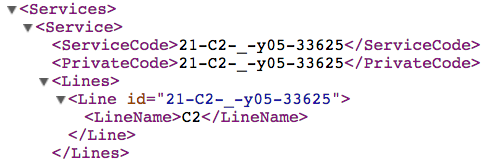
\includegraphics[width=\textwidth]{figures/xml_linename.png}
\caption{\label{fig:xml_linename} TfL Journey Planner Timtables XML LineName}
\end{figure}

\begin{figure}
\centering
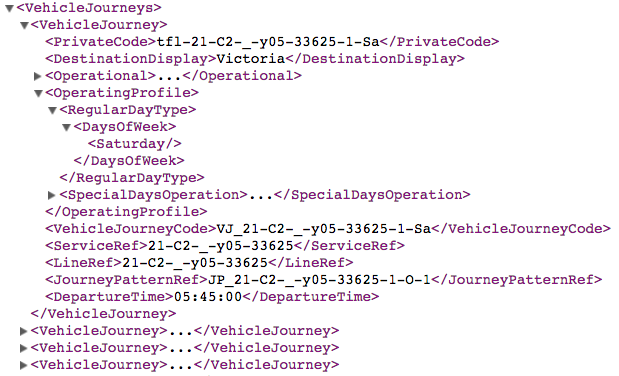
\includegraphics[width=\textwidth]{figures/xml_vehicle_journeys.png}
\caption{\label{fig:xml_vehicle_journeys} TfL Journey Planner Timtables XML VehicleJourney}
\end{figure}


\begin{figure}
\centering
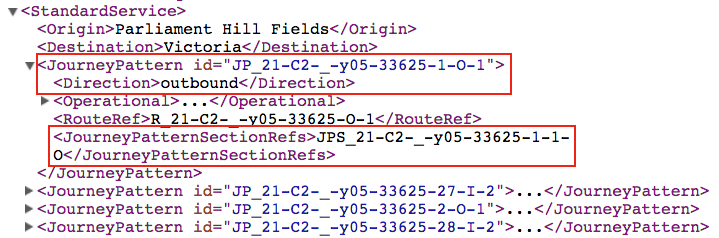
\includegraphics[width=\textwidth]{figures/xml_journeypattern.png}
\caption{\label{fig:xml_journeypattern} TfL Journey Planner Timtables XML JourneyPattern}
\end{figure}

\begin{figure}
\centering
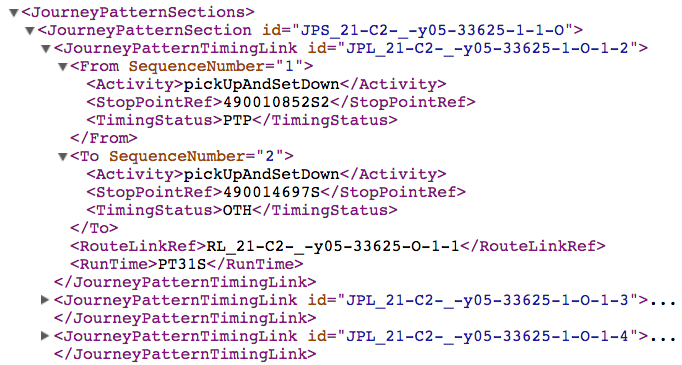
\includegraphics[width=\textwidth]{figures/xml_journey_pattern_section.png}
\caption{\label{fig:xml_journey_pattern_section} TfL Journey Planner Timtables XML JourneyPatternSection}
\end{figure}

\begin{figure}
\centering
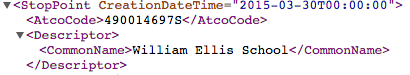
\includegraphics[width=\textwidth]{figures/xml_stoppoint.png}
\caption{\label{fig:xml_stoppoint} TfL Journey Planner Timtables XML StopPoint}
\end{figure}

\begin{enumerate}
  \item Obtain the route from \texttt{Services} $\rightarrow$ \texttt{Service} $\rightarrow$ \texttt{Lines} $\rightarrow$ \texttt{Line} $\rightarrow$ \texttt{LineName}, \textit{C2}. (Figure \ref{fig:xml_linename})
  \item For each \texttt{VehicleJourneys} $\rightarrow$ \texttt{VehicleJourney} (Figure \ref{fig:xml_vehicle_journeys}), extract the followings:
  \begin{enumerate}
    \item The departure time from \texttt{DepartureTime}, \textit{05:45:00}.
    \item The days of the week that this journey operates on from \texttt{OperatingProfile} $\rightarrow$ \texttt{RegularDayType} $\rightarrow$ \texttt{DaysOfWeek}, \textit{Saturday}.
    \item The corresponding journey pattern reference from \texttt{JourneyPatternRef}, \textit{JP\_21-C2-\_-y05-33625-1-O-1}.
  \end{enumerate}
  \item Each \texttt{JourneyPatternRef} maps to one Journey Pattern Section. This mapping is stored in \texttt{Services} $\rightarrow$ \texttt{Service} $\rightarrow$ \texttt{StandardService} $\rightarrow$ \texttt{JourneyPattern} (Figure \ref{fig:xml_journeypattern}).

  Retrieve the corresponding Journey Pattern Section Reference as such:
    \begin{enumerate}
      \item Each \texttt{JourneyPattern} element contains an element id, and a sub-element \texttt{JourneyPatternSectionRefs}.
      \item Map each Journey Pattern id to its corresponding \\ \texttt{JourneyPatternSectionRefs} for reference.
      \item Consult the above mapping to retrieve the Journey Pattern Section Reference for each Journey Pattern Reference found in Step 2(c). In the example case shown in Figure \ref{fig:xml_journeypattern}, \texttt{JourneyPattern} with \texttt{id=}\textit{JP\_21-C2-\_-y05-33625-1-O-1} has \texttt{JourneyPatternSectionRefs} \textit{JPS\_21-C2-\_-y05-33625-1-1-O}.
      \item Obtain the direction from the \texttt{Direction} sub-element. After comparing with the \acrshort{tfl} Bus Sequences data, we found out that \texttt{outbound} corresponds to run 1 and \texttt{inbound} corresponds to run 2.
    \end{enumerate}
    \item Next, obtain the bus travel time between every pair of neighbouring stops in the route from the \texttt{JourneyPatternSections} (Figure \ref{fig:xml_journey_pattern_section}). The detailed steps are as the following:
    \begin{enumerate}
      \item For each \texttt{JourneyPatternSectionRefs}, find the corresponding \texttt{JourneyPatternSections} $\rightarrow$ \texttt{JourneyPatternSection} with the same id, \textit{JPS\_21-C2-\_-y05-33625-1-1-O}.
      \item Each \texttt{JourneyPatternSection} contains multiple \\ \texttt{JourneyPatternTimingLink} sub-elements. Each sub-element contains information for one pair of neighbouring bus stops. Retrieve the following information from each sub-element:
      \begin{enumerate}
        \item \texttt{From SequenceNumber}, \textit{1}.
        \item \texttt{From} $\rightarrow$ \texttt{StopPointRef}, \textit{490010852S2}.
        \item \texttt{To SequenceNumber}, \textit{2}.
        \item \texttt{To} $\rightarrow$ \texttt{StopPointRef}, \textit{490014697S}.
        \item \texttt{RunTime}, \textit{31 seconds}.
      \end{enumerate}
    \end{enumerate}
    \item Each \texttt{StopPointRef} maps to a \texttt{StopPoints} $\rightarrow$ \texttt{StopPoint} $\rightarrow$ \texttt{AtcoCode} element. Each \texttt{StopPoint} element contains the stop name in its \texttt{Descriptior} element (Figure \ref{fig:xml_stoppoint}).

    For each \texttt{StopPointRef} obtained in step 4(b), retrieve the corresponding stop name as such:
    \begin{enumerate}
      \item Go through every \texttt{StopPoint} to build a map from \texttt{AtcoCode} to \texttt{Descriptior}.
      \item Consult the above mapping to retrieve the stop name for each \texttt{StopPointRef} found in step 4(b), \textit{William Ellis School}.
    \end{enumerate}

    \item After performing the above steps for every data point, we would have obtained the departure time from the terminal stop for each vehicle journey (Step 2(a)), and the bus travel time between every pair of the neighbouring stops (Step 4(b)v.). We calculated the cumulative bus travel time for each stop, and derived the bus arrival time at each stop for the given vehicle journey. We included a column \texttt{arrival\_hour} to store the hour that the arrival time falls in. This data is stored in the \texttt{delay\_tfl\_timetable\_archive} table. Figure \ref{fig:tfl_timetable_archive_sample} shows some sample entries from this table returned by the following SQL query.

    \begin{verbatim}
SELECT route, day, run, sequence, stop_name,
       naptan_atco, departure_time_from_origin,
       travel_time, cumulative_travel_time,
       arrival_time
FROM delay_tfl_timetable_archive
WHERE route='C2' AND day='Saturday'
      AND arrival_hour = 5 AND run = 1
ORDER BY sequence, departure_time_from_origin
    \end{verbatim}

\begin{figure}
\centering
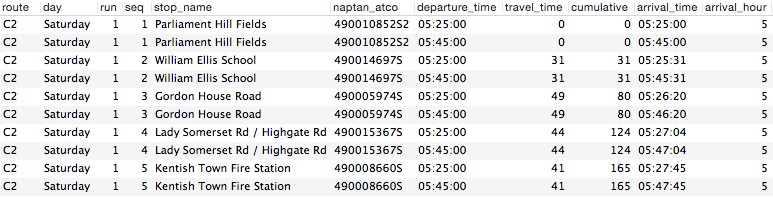
\includegraphics[width=\textwidth]{figures/tfl_timetable_archive_sample.png}
\caption{\label{fig:tfl_timetable_archive_sample} TfL Timtables Archive Sample}
\end{figure}

    \item As the \texttt{delay\_tfl\_timetable\_archive} table has more than 12 million entries, it was slow to run queries on it. Response time could go up to more than 20 seconds. In order to improve query performance, we further grouped the entries by \texttt{arrival\_hour}, and computed the average bus travel time between every pair of the neighbouring stops for the given hour of the given day of the week. This data was stored in the \texttt{delay\_tfl\_timetable} table (Schema shown in Table \ref{table:delay_tfl_timetable}) by running the following SQL statement. The resulting table has about 2.8 million entries and a query response time of about 5 seconds.

\begin{verbatim}
INSERT INTO delay_tfl_timetable
(route, day, run, sequence, stop_name,
naptan_atco, average_travel_time, arrival_hour)
(SELECT route, day, run, sequence, stop_name, naptan_atco,
        AVG(travel_time) as average_travel_time, arrival_hour
 FROM delay_tfl_timetable
 GROUP BY route, day, run, sequence, arrival_hour)
\end{verbatim}

    Figure \ref{fig:tfl_timetable_sample} shows sample average travel times for route C2 outbound journeys on Saturday morning 5am. We observed that there are less number of entries than the sample shown in Figure \ref{fig:tfl_timetable_archive_sample}.

\begin{figure}
\centering
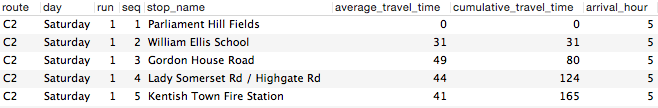
\includegraphics[width=\textwidth]{figures/delay_tfl_timetable_sample.png}
\caption{\label{fig:tfl_timetable_sample} TfL Timtables Sample}
\end{figure}

\end{enumerate}

The \acrshort{tfl} Reference Timetable is thus generated.




%!TEX root = report.tex
\section{Generating Current Timetable}
\label{sec:current_timetable_generation}

\subsection{Collecting Bus Arrival Times}
\label{sec:collecting_arrival_times}

\subsubsection{Building the Query URL}
\par We collect bus arrival data for analysis from the live bus arrivals API. The base URL used in this project was \url{http://countdown.api.tfl.gov.uk/interfaces/ura/instant_V1}.

\par We supplied the following parameters which specify the fields returned by the \acrshort{api}.

\begin{itemize}
  \item \textit{StopID} This is the alphanumeric identifier of a bus stop. It is also known as stop\_code\_lbsl.
  \item \textit{LineName} This is the route number that is displayed on the front of the bus on any publicity advertising the route.
  \item \textit{DirectionID} The direction of the bus.
  \item \textit{VehicleID} The unique identifier of the vehicle.
  \item \textit{TripID} The identifer of the specific trip that the prediction is for.
  \item \textit{EstimatedTime} This is the predicted time of arrival for the vehicle at a specific stop.
  \item \textit{ExpireTime} This is the time at which the corresponding prediction is no longer valid and should stop being displayed.
\end{itemize}

\par The resulting query URL is \sloppy \url{http://countdown.api.tfl.gov.uk/interfaces/ura/instant_V1?ReturnList=StopID,LineName,DirectionID,VehicleID,TripID,EstimatedTime,ExpireTime}.

\subsubsection{Storing Arrival Times}
\par The TfL Live Bus Arrival Feed is updated every 30 seconds to give a more accurate predictions of the bus arrival times. We send an HTTP request to the above URL every 30 seconds.

\par Each data entry in the return result contains an estimated arrival time for each bus journey at a given bus stop. We assume that the actual bus arrival time is the the midpoint between the last estimated arrival time, and the system time when the clear signal (\textit{ExpireTime} = 0) is received.

\par Since sometimes the clear signal is lost for certain entries, we will assume the actual bus arrival time is the last estimated arrival time, when it is more than 15 minutes after the expire time. This means that we have not received any new updates for the given bus at a given stop 15 minutes after the last estmated arrival time.

\par As we would like to only store the actual bus arrival times, we keep a local copy of the current query result using the pickle module in Python\cite{pickle}, and only update the Databases when the most arrival time for the given bus at the given stop has expired for more than 15 minutes.

\par We achieved this by the following steps:

\begin{enumerate}
  \item Load the local arrivals objects if there exists a copy.
  \item Pull the new TfL arrivals predictions.
  \item Update the loacl arrivals objects with the new predictions.
  \item For arrival entries that have expired for more than 15 minutes, remove these entries from the local copy, and store them in the delay\_arrivals table in the Databases.
\end{enumerate}

These steps were implemented in a Python script. Each run of the steps takes approximately 10 to 15 seconds. We re-run the script 15 seconds after the previous run finishes.

\subsection{Generating Bus Sequences and Neighbouring Stops}
\label{sec:bus_stop_locations_routes}
\par We imported the bus routes data introduced in Section \ref{sec:bus_sequence} into the delay\_bus\_sequences table (Table \ref{table:delay_bus_sequences}). Every entry contains information on the route name, route direction, and the sequences of stops in the route. As the sequence information for some routes have gaps, we preprocessed the data by updating the sequence number of the following stops to fill up the gaps. This preprocessing step was done after a few examples verified with the up-to-date TfL routes in the TfL Journey Planner.

\par In order to find out the average travel time between any pair of neighbouring stops, we need a list of all the neighbouring stops serving by various routes for reference.

\par We extracted this information from the bus routes data , and stored it in the delay\_neighbours table (Table \ref{table:delay_neighbours}). In the sample entries shown in Table \ref{table:sample_neighbours_view}, we can see that there are three different routes serving between stop 10002 and 11469. When calculating the average travel time between these two stops at a given hour, we used all bus trip information for these three routes.

\begin{table}
\centering
\begin{tabular}{@{}llrr@{}} \toprule
id & route & start\_stop & end\_stop \\ \midrule
18433 & 30 & 10002 & 11469 \\
44878 & N19 & 10002 & 11469 \\
8653 & 19 & 10002 & 11469 \\ \bottomrule
\end{tabular}
\caption{Sample data in delay\_neighbours Table}
\label{table:sample_neighbours_view}
\end{table}

\subsection{Generating the Current Average Travel Time Between Neighbouring Stops}
\par To generate the current average travel time, we first isolated the arrival times collected in the recent one hour.

\par We then performed the following steps on the recent arrivals data:

\begin{enumerate}
  \item For each bus traveling between each pair of the neighbouring bus stop,
  \begin{enumerate}
    \item We found out the arrival times for the same bus at the start stop and the end stop of the neighbouring pair.
    \item We calculated the difference of these two arrival times, and saved it as one entry of the travel time.
  \end{enumerate}
  \item We computed the the average travel time of all bus trips took place between every pair of neighbouring stops, and saved it in the current timetable.
  \item We also saved the current day of week, and hour of the day in the timetable for reference.
\end {enumerate}

\par We ran the above steps every hour to refresh the current timetable. Before every update, we stored the current timetable into a log for generating the historical timetable.


% \subsection{Negative Travel Time Filter}
% \par In the travel\_time\_log generated, there were trips between two neighbouring stops with negative travel times, such as the entry shown in Table \ref{table:travel_time_log_negative}.

% \begin{table}
% \centering
% \begin{tabular}{@{}lllllr@{}} \toprule
% Start Stop & End Stop & Route & Start Time & End Time & Travel Time(sec) \\ \midrule
% 9326 & 15552 & W13 & 14:53:18 & 14:52:14 & -64 \\ \bottomrule
% \end{tabular}
% \caption{Travel Time Log Entry with Negative Travel Time}
% \label{table:travel_time_log_negative}
% \end{table}

% \par This was because when we performed the join of the arrivals table, there was a more recent update on the arrival times for the start stop, whereas the arrival times of end stop had not been updated. In Table \ref{table:negative_travel_time_explained}, we observed that the Recorded Time for the end stop 9326 was more recent than that of the end stop. As a result, the arrival time for the end stop was earlier than the start stop, causing the travel time to be negative.

% \begin{table}
% \centering
% \begin{tabular}{@{}lllllr@{}} \toprule
% Stop Code & Route & Vehicle ID & Trip ID & Arrival Time & Recorded Time\\ \midrule
% 9326 & W13 & 18685 & 135229 &  14:53:18 & 14:48:25 \\ [0.4cm]
% 15552 & W13 & 18685 & 135229 & 14:52:14 & 14:44:02 \\ \bottomrule
% \end{tabular}
% \caption{Arrivals Entries to Explain Negative Travel Time}
% \label{table:negative_travel_time_explained}
% \end{table}

% \par We filtered out these negative values before calculating the average travel time between neighbouring stops.

%!TEX root = report.tex
\section{Generating Historical Timetable}
\label{sec:historical_timetable}
\par The historical timetable is generated from the current timetables. We processed the current timetable log by computing the average bus travel time by the start stop, end stop, day of the week, and hour of the day. This computation is performed weekly on Sunday midnight when the server is less busy to update the \texttt{delay\_historical\_timetable}. The following SQL script details the update task.

\begin{verbatim}
TRUNCATE delay_timetable_updated;

INSERT INTO delay_timetable_updated
(start_stop, end_stop, day, hour, average_travel_time)
(
  SELECT start_stop, end_stop, day, hour,
         AVG(average_travel_time) AS average_travel_time
  FROM delay_current_timetable_log
  GROUP BY start_stop, end_stop, day, hour
);

INSERT INTO delay_timetable
(start_stop, end_stop, day, hour, average_travel_time)
SELECT start_stop, end_stop, day, hour, average_travel_time
FROM delay_timetable_updated
ON DUPLICATE KEY UPDATE
delay_timetable.average_travel_time =
delay_timetable_updated.average_travel_time;
\end{verbatim}


\section{Summary}
\par The data collection and generation forms is the key stage to produce the reference, current, and historical timetables. After we crafted and tested the scripts and procedures to update the timetables, we proceeded to build the data service API. This is discussed in the next chapter.

%!TEX root = report.tex
\chapter{Delay Data Service}
\label{ch:data_service}
\section{Overview}
\par To enable structured query of the reference, current, and historical timetables, we created a REST data service \acrshort{api}. These endpoints are available within the imperial network for other developers to use.

\section{Django Framework}
\par We used Django Framework \cite{django_framework} for the backend of this project. It is a high-level Python Web framework that encourages rapid development and clean, pragmatic design. We chose it for the following advantages:

\begin{itemize}
  \item It stores databases schema as data models \cite{django_model}, and allows for quick database migration. This makes deployment to the production server easy by using the built-in migration command \cite{django_migrations}.
  % \item Django handles user authentication securely \cite{django_user_auth}, which saves work for development on this part.
  \item It has a compatible REST framework\cite{django_rest}, which supports REST API routing\cite{django_rest_routing} and query parameter parsing. Additionally, it offers a built-in user interface that displays the query result with pagination\cite{django_rest_pagination}.
  \item Django has a Debug mode that display constructive error messages, make the development much easier.
  \item It is written in Python, which is our preferred language for its simple and short syntax.
\end{itemize}

\section{Deployment Setup}
\subsection{Python Virtual Environment}
\par In order to manage our Python project requirements neatly and make deployment simple, we set up virtual environment\cite{virtualenv} \cite{virtualenvwrapper} to manage the project requirements. This helps to separate the Python packages installed for different projects as well.

\subsection{Web Server}
\label{sec:gunicorn}
We chose to use Nginx\cite{nginx} as the web server and Gunicorn\cite{gunicorn} as the Python Web Server Gateway Interface HTTP Server. Nginx was chosen over Apache Web Server as it was more widely used with Django and Gunicorn setup, therefore there was more support articles available online for reference \cite{nginx_gunicorn_django}.

\section{API Endpoints}
\par We built the backend using Django framework and Django REST framework, and exposed the following 3 endpoints for users to access data. The base URL for all endpoints is \url{http://delay.doc.ic.ac.uk:5000}.

%!TEX root = report.tex

\subsection{Historical \& Current Timetables}
\par This API endpoint is built to provide information on how long the bus on a given route at a given hour of the given day will take to reach the future stops from a given starting stop.

\subsubsection{Query URL \& Parameters}
\label{sec:predictions_params}
\par The base URL to access the historical and current timetables is \url{http://delay.doc.ic.ac.uk:5000/predictions/?}.

\par The following parameters are required to obtain a specific set of predictions:
\begin{itemize}
  \item \textbf{day} Day of the week
  \item \textbf{hour} Hour of the day [0 - 23]
  \item \textbf{route} Route
  \item \textbf{run} Route direction
  \item \textbf{naptan\_atco} The \gls{naptan} code for the starting downstream stops in the route
\end{itemize}

\par For example, the URL to retrieve historical and current bus travel time predictions for route 360 for downstream stops starting with \gls{naptan} code 490016263E at hour 15 on Tuesday is \url{http://delay.doc.ic.ac.uk:5000/predictions/?day=Tuesday&hour=15&route=360&run=2&naptan_atco=490016263E}.

\subsubsection{Result Format}
\par The result of the API query is a JSON list of bus stops, following the given route sequences in the given route direction, starting with the given stop.

\par Each bus stop entry contains information on the bus stop, as well as the bus travel time in seconds. The following four fields are the most important ones:

\begin{itemize}
  \item \textbf{average\_travel\_time} Historical average bus travel time from the previous stop to the current stop.
  \item \textbf{cumulative\_travel\_time} Historical average bus travel time from the given starting stop to the current stop.
  \item \textbf{average\_travel\_time} Current average bus travel time from the previous stop to the current stop.
  \item \textbf{cumulative\_travel\_time} Current average bus travel time from the given starting stop to the current stop.
\end{itemize}

\subsubsection{Backend Computation}
For each request, the Django backend performs the following computation steps to produce the response:

\begin{itemize}
  \item Search the database for the bus sequence with the given route and run.
  \item If a \gls{naptan} code is given, filter out the stops after the given stop.
  \item For each pair of the neighbouring stops, search the databases for the corresponding historical travel time, and the current travel time values for the give hour of the day, and day of the week.
  \item Compute the cumulative travel time from the starting stop to each downstream stop.
  \item Return the result in JSON format.
\end{itemize}

%!TEX root = report.tex

\subsection{Reference Timetable}
\par This API endpoint is designed to provide information on the \acrshort{tfl} official bus travel time for the buses on a given route at a given hour of the given day of week to reach downstream stops from a given starting stop.

\subsubsection{Query URL \& Parameters}
\par The base URL to access the reference timetable is \url{http://delay.doc.ic.ac.uk:5000/tfl_timetable/?}.

\par The required parameters are the same for the predictions endpoint, described in Section \ref{sec:predictions_params}.

\par For example, the URL to retrieve reference timetable entries for route 360 for downstream stops starting with \gls{naptan} code 490016263E at hour 15 on Tuesday is \url{http://delay.doc.ic.ac.uk:5000/tfl_timetable/?day=Tuesday&hour=15&route=360&run=2&naptan_atco=490016263E}.

\subsubsection{Result Format}
\par The result of this API query is similar to that of the prediction endpoint. It consists of a JSON list of bus stops, ordered by the given route sequences.

\par Each bus stop entry contains information on the bus stop. Additionally, the \textbf{average\_travel\_time} field indicates the official bus travel time from the previous stop to the current stop in seconds, whereas the \textbf{cumulative\_travel\_time} field shows the official bus travel time from the givien starting stop to the current stop in seconds.

\subsubsection{Backend Computation}
The backend processes each request as such:

\begin{itemize}
  \item Search the tfl timetable in databases for the entries for the given route, run and arrival hour.
  \item Filter the entries for the given day of the week, and the future stops of the given stop.
  \item Compute the cumulative travel time for the bus to reach each downstream stop from the given stop.
  \item Return the result in JSON format.
\end{itemize}



%!TEX root = report.tex
\subsection{Arrival}
\par This endpoint serves as a wrapper for the \acrshort{tfl} Live Bus API endpoint. Given a set of \acrshort{gps} coordinates and the radius of circle, this API endpoint returns the arrival times of buses arriving at stops within the circle.

\subsubsection{Query URL \& Parameters}
\par The base URL for this endpoint is \url{http://delay.doc.ic.ac.uk:5000/arrivals/?}. The required parameters include the latitude and the longitude of the \acrshort{gps} coordinates, and the radius in meters. An example query URL would be \url{http://delay.doc.ic.ac.uk:5000/arrivals/?latitude=51.495171603309615&longitude=-0.1883983612060547&radius=100}.

\subsubsection{Result Format}
\par The query result is a list of bus stops within the circle. Each bus stop entry has basic information about the stop, and a list of the buses arriving at the stop in the next 30 minutes, grouped by the bus routes. Within each route, the \texttt{estimatedTimeInSeconds} shows the arrival times of the buses arriving at the given stop. See Figure \ref{fig:arrival_api} for example response.


\begin{figure}
\centering
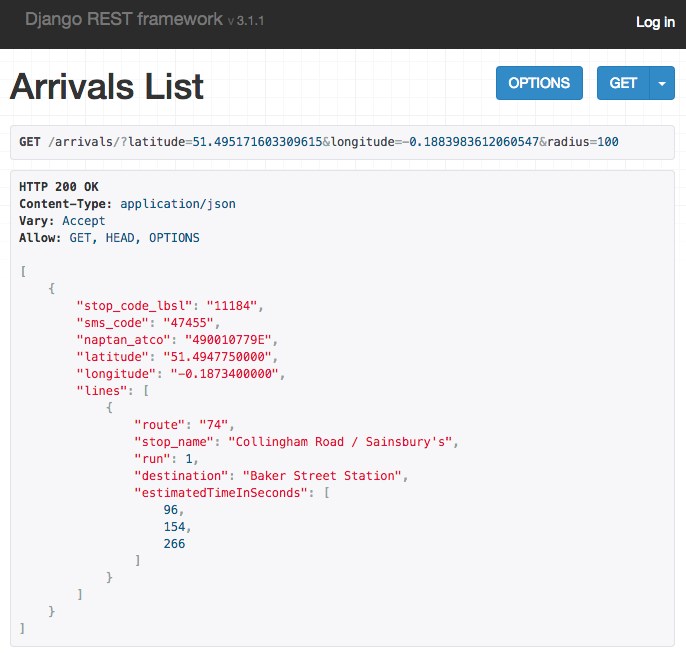
\includegraphics[width=\textwidth]{figures/arrival_api.png}
\caption{\label{fig:arrival_api} Sample Response for Arrivals API}
\end{figure}

\section{Summary of Data Service API}
Building these three API endpoints enabled us to meet the first objective by supplying data on bus travel time predictions. We evaluated the accuracy and performance in Chapter \ref{ch:evaluation}.

%!TEX root = report.tex
\chapter{WebApp for Active Delay Warning}
\label{ch:mobile_app}

\par We designed a web application to demonstrate the potential use of our API data service. It allows users to search for nearby bus stops, view the available routes and live bus arrival times. For each route, the user can view the historical, current and reference bus travel time to reach each downstream bus stop.

\section{Implementation}
\subsection{AugularJS Framework}
\par We chose to use the AngularJS Framework \cite{angularjs} with UI Bootstrap \cite{bootstrap} to build the frontend of the application. This was because AngularJS employs a clear Model-View-Controller structure, and has a wide range of packages to build extensions with.

\subsection{Development \& Deployment Pipeline}
\par We used Yeoman \cite{yeoman}, a web application scaffolding tool, to organise and manage scripts and files. We also used Grunt \cite{grunt}, a Javascript task runner to manage the build and delopment process.

\par For deployment, we created a Grunt task to run tests, minify the javascript files, and copy the minified version to the production server.

\section{Frontend Walkthrough}
\par We deployed the frontend web to \url{http://delay.doc.ic.ac.uk/}.

\todo[inline]{insert 3 screenshots}

\subsection{Landing Page}
\par The map will be centered at the current location of the device. If the current location is not available, then the default map centered on London will be loaded.

\subsection{Nearby Bus Stops Arrival}
\par A click on the map will place a grey location marker and make a request to search for the nearby bus stops within a given radius. The default radius is 100 meters.

\par A list of the nearby bus stops and the routes available at each stop will be shown, with the \acrshort{tfl} bus arrivals predictions shown.

\subsection{Bus Delay Predictions}
\par We could check the historical, current, and reference travel time to each downstream stops by selecting a specific route for details. There is likely delay when the current bus travel time is more than the reference bus travel time.

\section{Summary}
\par The web application shows how the delay prediction data service could be used to inform users of potential delays in buses arriving at any downstream stops on a selected route. This will help bus passengers to make informed decisions when choosing travel mode and bus routes to save time.


%!TEX root = report.tex
\chapter{Other Technical Details}


\section{Daemen Script Management - Supervisor}

\section{Scheduled Tasks Management - Jenkins}
\par We used Jenkins\cite{jenkins} to managed our predictions timetable update schedule.
\todo[inline]{add screenshots for jenkins}


\subsection{Current Timetable Update}
\par The current timetable is re-generated every hour. We set up a Jenkins job to re-run the relevant current timetable update SQL script every hour, and save the previous timetable into a log for updating the historical timetable at a later time. This job takes less than 10 minutes on average.

\subsection{Historical Timetable Update}
\par Similarly, we set up a Jenkins job to update the Historical Timetable daily at 3.30am when the server is less busy.

\subsection{Arrivals Daily Backup}
\par The arrivals table grows rapidly by approximately 150 thousand rows per hour. In order to allow fast access to the arrivals within the past one hour to construct the current timetable, we decided to save the arrivals for the current day in a new table, while keeping the past arrivals entries in an archive table. This required us to backup the arrivals entries daily to the arive.

\par Again, we created a Jenkins job to run the back up script daily. In order not to affect the historical timetable update, we set this job as a downstream task of the historical timetable update.

\subsection{Software Project Management - Trello}
\par We used Trello \cite{trello} for project management. It was useful to keep track of the tasks backlog, the tasks at hand, and the tasks to be further tested (Figure \ref{fig:trello}).

\begin{figure}
\centering
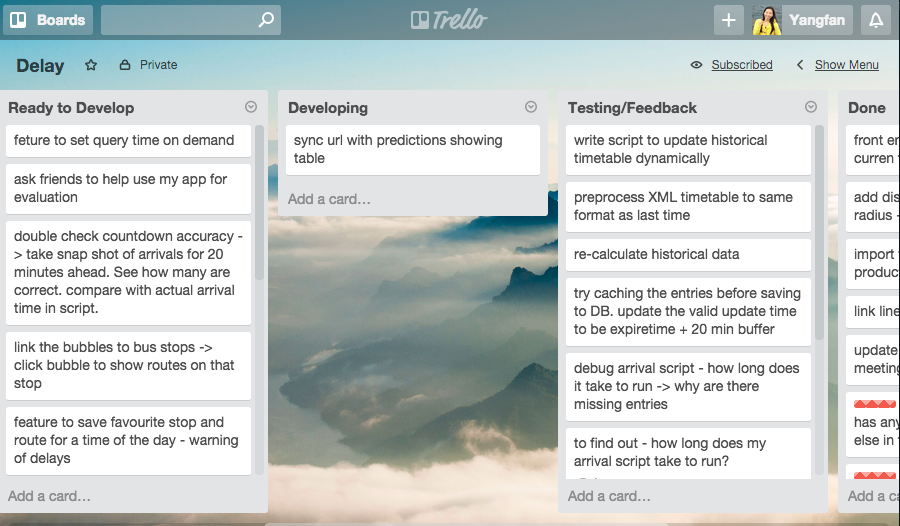
\includegraphics[width=\textwidth]{figures/trello_small.png}
\caption{\label{fig:trello} Project Trello Board}
\end{figure}

% %!TEX root = report.tex
\chapter{Project Plan}

\section{Project Objectives}
This project aims to produce a tool that notifies users of delays of the London buses they are waiting for, so that they can choose alternate routes and save waiting time.

\begin{description}
	\item[Back-end]  A timetable of bus journey times with an interface that supports real time query.
    \item[Front-end] A mobile application that allows users to check bus arrivals times with delay information at a give time and location.
\end{description}

\subsection{Core Features}
    \begin{enumerate}
        \item Given user current location, query for predicted bus arrivals at the nearest bus stop.
 		\item Give user current location and destination, query for routes and suggest bus routes with delays taken into consideration.
        \item Given starting location, destination, desired departure / arrival time, suggest bus routes with delays taken into consideration.
    \end{enumerate}

\subsection{Optional Extensions}
    \begin{enumerate}
    	\item Optimise prediction accuracy
        	\begin{itemize}
            	\item Analyse the average bus journey time for given starting and end stops to remove outliers.
                \item Integrate iBus actual arrivals data to improve arrivals timetable precision.
            \end{itemize}
        \item Include other modes of transportation for alternate route recommendation.
        \item Gather more user feedback on mobile application and improve accordingly .
        \item Publish mobile application on android market.
    \end{enumerate}

\section{Current Progress}
\begin{enumerate}
  \item Obtained access to TFL Live bus arrival API stream.
  \item Designed databases schema.
  \item Setup databases to store bus arrival data.
  \item Setup remote server to run daemon process to pull data from live bus arrivals feed and store data into the database.
  \item Collected 2 weeks of bus arrivals data for analysis.
  \item Created sample bus arrivals timetable for a chosen pair of neighbouring bus stops (10002 - 11469).
\end{enumerate}

\section{Development Plan}
\begin{description}
	\item \textbf{Spring Term Week 4}
    \begin{itemize}
    	\item Optimise arrivals table for fast query (e.g. via proper indexing).
		\item Create bus journey timetables with delay for all pairs of neighbouring bus stops.
    \end{itemize}
    \item \textbf{Spring Term Week 5}
    Develop journey planning feature with given start and end stops
    \item \textbf{Milestone 1 - Spring Term Week 6}
    Design query to request journey time from bus stop A to bus stop B at a given time of the day.

	\item \textbf{Spring Term Week 7}
    \begin{itemize}
    	\item Develop back-end API to receive query from mobile application.
    	\item Start initial mobile interface design.
    \end{itemize}
	\item \textbf{Spring Term Week 8}
	Design mobile application interface to extract user current location, and identify the nearest bus stop.
    \item \textbf{Milestone 2 - Spring Term Week 9}
    Connect mobile application to send query to the back-end to request for bus arrival times for all routes reaching ther nearest bus stop.
    \item \textbf{Spring Term Week 10}
    Improve mobile application user interface (gain user feedback and improve incrementally).
	\item \textbf{Fall-back Point - Easter Break}
    \begin{itemize}
    	\item Implement mobile interfaces to get journey destination for journey planning.
        \item Display suggested journey routes and travel time for a give time.
    	\item Optimise delay predictions by filtering out anomalies in average journey time calculation
    	\item Evaluate performance by comparing with iBus data
    \end{itemize}
    \item \textbf{Milestone 3 - Summer Term Week 1 - 3} Implement extensions and start writing report.
	\item \textbf{Summer Term Week 4} Report first draft.
    \item \textbf{Summer Term Week 5} Report second draft.
    \item \textbf{Summer Term Week 6} Presentation first draft.
    \item \textbf{Summer Term Week 7} Presentation second draft.
    \item \textbf{Summer Term Week 8}
    	\begin{itemize}
        	\item \textbf{Tuesday, 16th June 4pm} Final report due.
    		\item Presentation practice.
        \end{itemize}
    \item \textbf{Summer Term Week 9, Monday 22nd and Tuesday 23rd June} Presentation days.
    \item \textbf{Summer Term Week 10, Monday 29th June} Final Archive due.
\end{description}
%!TEX root = report.tex
\chapter{Evaluation}
\label{ch:evaluation}
\section{Accuracy of Live Bus Arrivals API Stream}
\par The Tfl Live Bus Arrivals API Stream updates the bus arrival times every 30 seconds. This means that the bus arrival predictions for the current stop would get more and more accurate as the bus approaches the stop. This is because any error in earlier predictions would be incrementally corrected at every update as the location of the bus gets refreshed.

\subsection{Test for Accuracy}
\par We evaluated the accuracy of these predictions by the following steps:

\begin{itemize}
  \item We took a snapshot of all the bus arrivals predictions for the next 30 minutes at a given recorded time (2015-06-04 11:24:37).
  \item We grouped these prediciton entries by the difference between the predicted arrival time and the recorded time at a 5-minute interval. For example, the predictions for the buses arriving in the next 5 minutes, next 5 to 10 minutes, and next 10 to 15 minutes, etc. We added an additional group for the next 0 - 3 minutes for reference.
  \item After 3 hours, we compared each arrival prediction entry in the snapshot table against the actual arrival data we stored for generating the current timetable. The difference between the predicted and the actual arrival time gives an indication of the prediction accuracy. We stored this difference as the delta value. A negative delta indicates the bus came later than the predicted time.
  \item We calcuated the average delta value for each group, and created Table \ref{table:countdown_evaluation}.
\end{itemize}

\begin{table}
\centering
\begin{tabular}{@{}lr@{}} \toprule
Predictions for & Average Delta (Seconds) \\ \midrule
next 0 - 3 mintues & -34.8112 \\
next 0 - 5 mintues & -45.4951 \\
next 5 - 10 mintues & -97.2584 \\
next 10 - 15 mintues & -134.3606 \\
next 15 - 20 mintues & -169.5990 \\
next 20 - 25 mintues & -174.7177 \\
next 25 - 30 minutes & -166.1368 \\
\bottomrule
\end{tabular}
\caption{Live Bus Arrivals API Stream Accuracy - A negative delta indicates the bus came later than the predicted time}
\label{table:countdown_evaluation}
\end{table}

\subsection{Test Result}
\par Table \ref{table:countdown_evaluation} shows that buses usually came later than the predictions provided by the Live Bus Arrivals API Stream. For the buses that were predicted to due in the next 5 minutes, they usually came less than one minute later than the predicted arrival time. We took this finding into consideration when testing the accuracy of our current and historical timetable by only choosing buses that are due within the next 5 minutes as tracking targets.

\section{Correctness and Performance of the API}
\subsection{Tool}
\par We used \textit{siege}\cite{siege} to conduct the load test of our API endpoints. Our aim was to test the number requests the server could handle reliably at one time, and the response time it took.

\par \textit{Siege} takes in the number of users, the delay time between each page load, the test running time, and the list of URLs to send requests to as parameters. It then simulates the user behaviours to fire requests to the list of given URLs. At the end of the test, \textit{Siege} generates a report for the test, including metrics such as the transaction rate, and the response time of the target URLs.

\subsection{Preparation}
\par We generated a list of API URLs with random parameters for testing. We then ran the siege tests by fixing the test running time to be 1 minute, with 1 second of delay between each page load.

\subsection{Test for Correctness}
\par We first tested for the correctness of our API endpoints. This involves firing requests with random day of the week and hour of day, route, run, and starting bus stop code to check whether the server can return a response correctly.

\par At this stage, we found some specific URLs that resulted in a 500 error code, and debugged the backend code to return correct results. For example, this happened when we requested for a reference travel time for a bus route at an hour out of its operating time. As there was no corresponding entry in the databases, we fixed the code by returning an empty list by default.

\par After we received 200 status code for all requests in a few test runs consistently, we proceeded to perform the load tests by fixing the day of the week and hour of the day to be the current values when the test was run.

\subsection{Load Test for Performance}
\par We found out that currently, the server could reliably handle about 150 users to send requests concurrently, with an average response time of 15.78 seconds. Figure \ref{fig:performance} shows the results of our tests.

\begin{figure}
\centering
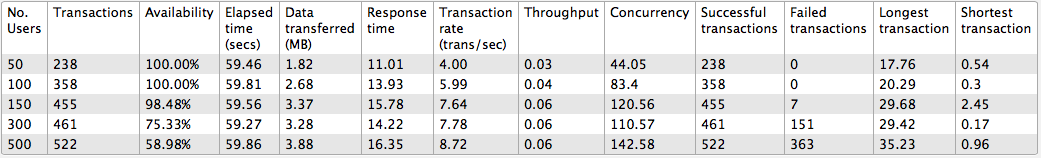
\includegraphics[width=\textwidth]{figures/performance.png}
\caption{\label{fig:performance} Result of Performance Test with Siege}
\end{figure}

\todo[inline]{plot graph from results}

\begin{verbatim}
Transactions is the number of server hits. In the example, 25 simulated users [ -c25 ] each hit the server with 10 repetitions [ -r10 ], a total of 250 transactions.

Elapsed time is the duration of the entire siege test. This is measured from the time the user invokes siege until the last simulated user completes its transactions. Shown above, the test took 14.67 seconds to complete.

Data transferred is the sum of data transferred to every siege simulated user. It includes the header information as well as content. Because it includes header information, the number reported by siege will be larger then the number reported by the server. In internet mode, which hits random URLs in a configuration file, this number is expected to vary from run to run.

Response time is the average time it took to respond to each simulated user’s requests.

Transaction rate is the average number of transactions the server was able to handle per second, in a nutshell: transactions divided by elapsed time.

Throughput is the average number of bytes transferred every second from the server to all the simulated users.

Concurrency is average number of simultaneous connections, a number which rises as server performance decreases.

Successful transactions is the number of times the server returned a code less then 400. Accordingly, redirects are considered successful transactions.
\end{verbatim}

\section{Accuracy of Predictions}
How accurate are the predictions?
\subsection{Compare predictions to real data}
We can compare the predictions generated to the live bus arrivals data stored in the arrivals table. We can calculate the standard deviation of the difference in the predicted time and actual arrival time. This value will be the direct indicator of the accuracy of the predictions.


\section{User feedback on UI}
\par On the
How effective is it at warning delay?


%!TEX root = report.tex
\chapter{Future Work}
\par Future work for this project mainly involves the following 3 aspects.
\label{ch:future_work}
\begin{enumerate}
  \item \textbf{API Performance}
\par Currently, only one server is used for data collection, timetable generation, and live \acrshort{api} query handling. This could be the cause of the long response time. The performance of the API endpoints could be improved by using at least two servers, one in charge of data collection and processing, and the other handle live user queries. When the user base grow in the future, we could also setup more servers to process the requests concurrently.

\item \textbf{Prediction Accuracy}
\par The accuracy of the bus journey time predictions could be further tested and improved by applying more advanced analytical methods. These include but not limit to the approaches presented in the literature review (Section \ref{sec:literature}).
% refactor
% into separate components
% make it less tightly coupled
% data collection \& pre-processing
% server handling live user queries

\item \textbf{WebApp Extensions}
\par We could inclue features to alert users of bus delays actively for extension. The application should track the device location, and alert users of any delays occurred on the frequently travelled routes. The user interface could be furture improve the make the experience smoother. For example, a blue dot could be added to the map to indicate the current location of the device, and be updated constantly. Additionally, bus journey planning and the ability to search start and end stops are also helpful.
\end{enumerate}



%!TEX root = report.tex
\chapter{Conclusion}

\par In this project, we built a data service to provide the average bus travel time for each downstream stop for a given route on a given day of the week and hour of the day. This prediction data API can support about 100 simultaneous users.

\par We also designed a demonstrative web application to showcase the potential use of the data service.


%!TEX root = report.tex
\begin{appendices}
\chapter{Database Table Schema}
\begin{table}
\centering
\begin{tabular}{@{}llr@{}} \toprule
Column Name & Type & Default \\ \midrule
id(Primary) & int(11) & Auto Increment \\
stop\_code\_lbsl & varchar(64) &  \\
route & varchar(64) &  \\
vehicle\_id & varchar(64) & \\
trip\_id & varchar(64) & \\
arrival\_date & date &  \\
arrival\_time & timestamp & NULL \\
expire\_time & timestamp & NULL \\
recorded\_time & timestamp & Current Timestamp \\ \bottomrule
\end{tabular}
\caption{delay\_arrivals Table Schema}
\label{table:delay_arrivals_schema}
\end{table}

\begin{table}
\centering
\begin{tabular}{@{}llr@{}} \toprule
Column Name & Type & Comments\\ \midrule
id(Primary Key) & int(11)  & Auto Increment\\
route & varchar(64) &  The route name\\
run & int(11) & The route direction\\
sequence & int(11) & The sequence of the bus stop in the route\\
stop\_code\_lbsl & varchar(64) & The internal bus stop identifier\\
bus\_stop\_code & varcher(64) & The public code for the bus stop\\
naptan\_atco & varchar(64) & The national identifier of the bus stop\\
stop\_name & varchar(64) & The name of the bus stop\\ \bottomrule
\end{tabular}
\caption{delay\_bus\_sequences Table Schema}
\label{table:delay_bus_sequences}
\end{table}


\begin{table}
\centering
\begin{tabular}{@{}llr@{}} \toprule
Column Name & Type & Comments\\ \midrule
id(Primary Key) & int(11)  & Auto Increment\\
route & varchar(64) & The bus route \\
start\_stop & varchar(64) & The stop\_code\_lbsl for the start stop\\
end\_stop & varcher(64) & The stop\_code\_lbsl for the end stop\\ \bottomrule
\end{tabular}
\caption{delay\_neighbours Table Schema}
\label{table:delay_neighbours}
\end{table}
\end{appendices}

\begin{table}
\centering
\begin{tabular}{@{}llp{6cm}@{}} \toprule
Column Name & Type & Comments\\ \midrule
id(Primary Key) & int(11)  & Auto Increment\\ [0.4cm]
route & varchar(64) & The bus route \\ [0.4cm]
day & varchar(32) & The day of week for the vehicle journey \\ [0.4cm]
run & int(11) & The route direction \\ [0.4cm]
sequence & int (11) & The sequence of the bus stop in the route \\ [0.4cm]
stop\_name & varchar(64) & The name of the bus stop \\ [0.4cm]
naptan\_atco & varchar(64) & The national identifier of the bus stop \\ [0.4cm]
average\_travel\_time & datetime(6) & The average travel time in seconds for the bus trips from the previous stop in the route to the current stop during the given arrival hour \\ [0.4cm]
cumulative\_travel\_time & int(11) & The average travel time in seconds from the terminal to the current stop for the bus trips arrived at the current stop in the given arrival hour \\
\bottomrule
\end{tabular}
\caption{delay\_tfl\_timetable Table Schema}
\label{table:delay_tfl_timetable}
\end{table}



\printglossary[type=\acronymtype]
\printglossary
% %!TEX root = report.tex

\cleardoublepage
%\pagebreak
\phantomsection
\addcontentsline{toc}{chapter}{References}
\begin{thebibliography}{99}

\bibitem{tfl_annual_report_13/14} Transport for London Annual Report and Statement of Accounts 2013/14, \
\url{http://tfl.gov.uk/cdn/static/cms/documents/annual-report-2013-14.pdf} [visited on 27/01/2015]

\bibitem{live_bus_arrivals} Transport for London Live Bus Arrivals, \
\url{http://www.tfl.gov.uk/modes/buses/live-bus-arrivals} [visited on 27/01/2015]

\bibitem{google_maps} Google Maps, \
\url{https://www.google.co.uk/maps} [visited on 30/01/2015]

\bibitem{citymapper} CityMapper, \
\url{https://citymapper.com/london} [visited on 30/01/2015]

\bibitem{tfl_journey_planner} TfL Plan A Journey, \
\url{http://tfl.gov.uk/plan-a-journey/} [visited on 30/01/2015]

\bibitem{buses_performance_report} Transport for London Buses Network Performance Second Quarter 2014/15, \
\url{http://tfl.gov.uk/cdn/static/cms/documents/network-performance-latest-quarter.pdf} [visited on 27/01/2015]

\bibitem{tfl_ltds} Travel in London, Supplementary Report: London Travel Demand Survey (LTDS), \
\url{http://www.tfl.gov.uk/cdn/static/cms/documents/london-travel-demand-survey.pdf} [visited on 28/01/2015]

\bibitem{bus_stop_locations_routes} Transport for London Bus Stops Locations and Routes Open Data\
\url{https://www.tfl.gov.uk/info-for/open-data-users/our-feeds} [visited on 28/01/2015]

\bibitem{open_data} Transport for London Open Data\
\url{https://www.tfl.gov.uk/info-for/open-data-users/our-open-data} [visited on 28/01/2015]

\bibitem{live_bus_api_documentation} Transport for London Live Bus \& River Bus Arrivals API Interface Documentation\
\url{https://www.tfl.gov.uk/cdn/static/cms/documents/tfl-live-bus-river-bus-arrivals-api-documentation-v16.pdf} [visited on 28/01/2015]

\bibitem{buses_performance_data} Transport for London Buses Performance Data\
\url{https://www.tfl.gov.uk/corporate/publications-and-reports/buses-performance-data#on-this-page-5} [visited on 28/01/2015]

\end{thebibliography}
\end{document}
